\documentclass{exercisesheet}

\resources{res}

\title{Aufgaben für Rechnerstrukturen \& Betriebssysteme}
\author{Leopold Lemmermann}
\solutions

\begin{document}
\createtitle

\exercisesheet{2020}{Ersttermin}
  \begin{exercise}{Zahlensysteme}
    \item Wandeln Sie die Dezimalzahl $N = 1956$ in eine 16-stellige Binärzahl um.
    \item Wie lautet die Darstellung von $N$ im Oktalsystem.
    \item Wie lautet die Darstellung von $N$ im Hexadezimalsystem.
    \item Wie lautet jeweils die Darstellung der negativen Zahl $N$ im Hexadezimalsystem (4 Stellen), wenn mit einer Angabe negativer Zahlen
      \begin{itemize}
        \item mit Vorzeichen/Betrag:
        \item Einerkomplementdarstellung:
        \item Zweierkomplementdarstellung:
      \end{itemize}
      gearbeitet wird.
  \end{exercise}

  \begin{solution}
    \item $N = 1956_{10} = {0000\ 0111\ 1010\ 0100}_2$
    \item $N = 1956_{10} = {3644}_8$
    \item $N = 1956_{10} = {\mathrm{07A4}}_{16}$
    \item $-N = -1956_{10} = $
      \begin{itemize}
        \item ${\mathrm{F7A4}}_{16}$
        \item ${\mathrm{F85B}}_{16}$
        \item ${\mathrm{F85C}}_{16}$
      \end{itemize}
  \end{solution}

  \begin{exercise}{Kommazahlen zwischen Basen}
    \item Wandeln Sie die Dezimalzahl $N = 0.85$ in eine (möglicherweise periodische) Binärzahl mit 4 Vorkomma- \& der Zahl Nachkommastellen um.
    \item Wie lautet die Darstellung von $N$ im Hexadezimalsystem?
    \item Wie wird $N$ im Zweierkomplement mit 4 Vorkomma- \& 8 Nachkommastellen codiert?
  \end{exercise}

  \begin{solution}
    \item $N = 0.85_{10} = {0000.11\overline{01\ 10}}_2$
    \item $N = 0.85_{10} = {\mathrm{.D\bar{9}}}_{16}$
    \item ${N}_{2K} = (0.85_{10})_{2K} = {1111.0010\ 0111}_2$
  \end{solution}

  \begin{exercise*}{Rechnen im Hexadezimalsystem}
    Gegeben seien die Hexadezimalzahlen $A = \mathrm{4B2F}$ und $B = \mathrm{3B32}$.
    \begin{enumerate}
      \item Addieren Sie $A+B$.
      \item Subtrahieren Sie $A-B$.
      \item Multiplizieren Sie $A\cdot (20)_{16}$.
    \end{enumerate}
  \end{exercise*}

  \begin{solution}
    \item $A + B = \mathrm{4B2F} + \mathrm{3B32} = \mathrm{8661}$
    \item $A - B = \mathrm{4B2F} - \mathrm{3B32} = \mathrm{0FFD}$
    \item $A \cdot B = \mathrm{4B2F} \cdot 20 = \mathrm{965E}$
  \end{solution}

  \begin{exercise*}{Umwandlung von IEEE-754 Gleitkommazahlen}
    Wandeln Sie die folgenden normalisierten 32-bit Gleitkommazahlen im IEEE-754 float-Format (1-bit Vorzeichen, 8-bit Exponent in Exzess-127 Darstellung, 23-bit Mantisse) in Dezimalzahlen um. Dabei sind nur die oberen 7 Bit der Mantisse angegeben (alle anderen Bits sind 0).
    \begin{itemize}
      \item $(0|0000 0000|0000 000)$:
      \item $(1|1000 0010|1110 000)$:
      \item $(0|0111 1111|0000 000)$:
      \item $(0|0111 1110|1000 000)$:
      \item $(1|0111 1111|0100 000)$:
    \end{itemize}
  \end{exercise*}

  \begin{solution*}
      \begin{itemize}
        \item $0.0$
        \item $-15.0$
        \item $1.0$
        \item $0.75$
        \item $-1.25$
      \end{itemize}
  \end{solution*}

  \begin{exercise*}{Codierung}
    Nachfolgend sind alle 4 Codewörter eines Codes angegeben:
    \begin{center} $w_1 = 0000001$, $w_2 = 0001110$, $w_3 = 1110000$, $w_4 = 1111111$ \end{center}
    \begin{enumerate}
      \item Bestimmen Sie den minimalen Hamming-Abstand der Codewörter.
      \item Welche Aussagen sind zutreffend?
        \begin{itemize}
          \item Es handelt sich um einen Binärcode.
          \item Es handelt sich um einen Blockcode.
          \item Es handelt sich um einen linearen Code.
          \item Es handelt sich um einen zyklischen Code.
          \item Mit dem Code können 2-bit Fehler erkannt werden.
          \item Mit dem Code können 3-bit Fehler erkannt werden.
          \item Mit dem Code können 1-bit Fehler korrigiert werden.
          \item Mit dem Code können 2-bit Fehler korrigiert werden.
          \item Mit dem Code können 1-bit Fehler korrigiert und 2-bit Fehler erkannt werden.
        \end{itemize}
    \end{enumerate}
  \end{exercise*}

  \begin{solution}
    \item $d_{min} = 4$
    \item Zutreffende Aussagen:
      \begin{itemize}
        \item Es handelt sich um einen Binärcode. \checkmark
        \item Es handelt sich um einen Blockcode. \checkmark
        \item Es handelt sich um einen linearen Code. \checkmark
        \item Es handelt sich um einen zyklischen Code. \checkmark
        \item Mit dem Code können 2-bit Fehler erkannt werden. \checkmark
        \item Mit dem Code können 3-bit Fehler erkannt werden. \checkmark
        \item Mit dem Code können 1-bit Fehler korrigiert werden. \checkmark
        \item Mit dem Code können 2-bit Fehler korrigiert werden. \xmark
        \item Mit dem Code können 1-bit Fehler korrigiert und 2-bit Fehler erkannt werden. \checkmark
      \end{itemize}
  \end{solution}

  \begin{exercise*}{Codierung nach Fano \& Huffman}
    Gegeben sei eine Menge $M = \{A, B, C, D, E\}$ von Symbolen, die mit folgenden Wahrscheinlichkeiten auftreten:
    \begin{center}
      \begin{tabular}{c|ccccc}
        $m_i$ & $A$ & $B$ & $C$ & $D$ & $E$\\
        \hline
        $p_i$ & 0,35 & 0,15 & 0,2 & 0,18 & 0,12\\
      \end{tabular}
    \end{center}
    \begin{enumerate}
      \item Geben Sie eine optimale Codierung der Elemente von $M$ nach Fano an.
      \item Geben Sie eine optimale Codierung der Elemente von $M$ nach Huffman an.
      \item Schreiben Sie die Formel auf, nach der die Entropie $H$ berechnet wird \& setzen Sie die Zahlen ein. Die Berechnung des Zahlenwertes entfällt.
    \end{enumerate}
  \end{exercise*}

  \begin{solution}
    \item
      \begin{tabular}{c|ccccc}
        $m_i$ & $A$ & $B$ & $C$ & $D$ & $E$\\
        \hline
        $p_i$ & 0,35 & 0,15 & 0,2 & 0,18 & 0,12\\
        $c_i$ & 00 & 10 & 01 & 11 & 001\\
      \end{tabular}
    \item
      \begin{tabular}{c|ccccc}
        $m_i$ & $A$ & $B$ & $C$ & $D$ & $E$\\
        \hline
        $p_i$ & 0,35 & 0,15 & 0,2 & 0,18 & 0,12\\
        $c_i$ & 0 & 110 & 10 & 111 & 111\\
      \end{tabular}
    \item
      \begin{equation*}
        \begin{split}
          H &= -\sum_{i=1}^{n} p_i \cdot \log_2(p_i)\\
          &= -(.35\cdot \log_2{.35}+ .15\cdot \log_2{.15}+ .2\cdot \log_2{.2}+ .18\cdot \log_2{.18}+ .12\cdot \log_2{.12})\\
          (&=2.18)
        \end{split}
      \end{equation*}
  \end{solution}

  \begin{exercise*}{Logische Funktionen}
    Gegeben sei die folgende logische Funktion $F$:
    \begin{center}
      \begin{tabular}{c|cccc cccc cccc cccc}
        $b_0$ & 0 & 1 & 0 & 1 & 0 & 1 & 0 & 1 & 0 & 1 & 0 & 1 & 0 & 1 & 0 & 1\\
        $b_1$ & 0 & 0 & 1 & 1 & 0 & 0 & 1 & 1 & 0 & 0 & 1 & 1 & 0 & 0 & 1 & 1\\
        $a_0$ & 0 & 0 & 0 & 0 & 1 & 1 & 1 & 1 & 0 & 0 & 0 & 0 & 1 & 1 & 1 & 1\\
        $a_1$ & 0 & 0 & 0 & 0 & 0 & 0 & 0 & 0 & 1 & 1 & 1 & 1 & 1 & 1 & 1 & 1\\
        \hline
        $F$ & 1 & 0 & 0 & 0 & 1 & 1 & 0 & 0 & 1 & 1 & 1 & 0 & 1 & 1 & 1 & 1 \\
      \end{tabular}
    \end{center}
    \begin{enumerate}
      \item Übertragen Sie $F$ in ein 4x4 KV-Diagramm.
      \item Finden Sie geeignete Schleifen \& geben Sie die minimale konjunktive Form von $F$ als logische Funktion $a_1, a_0, b_1, b_0$ an.
      \item Wie lautet die minimale disjunktive Form von $F$?
      \item Welche Vergleichsoperation der 2-bit Zahlen $(a_1a_0)$ \& $(b_1b_0)$ beschreibt $F$?
    \end{enumerate}
  \end{exercise*}

  \begin{solution}
    \item
      \begin{tabular}{c|cccc}
        $b_1b_0 \backslash a_1a_0$ & 00 & 01 & 11 & 10\\
        \hline
        00 & 1 & 1 & 1 & 1\\
        01 & 0 & 1 & 1 & 1\\
        11 & 0 & 0 & 1 & 1\\
        10 & 0 & 0 & 0 & 1\\
      \end{tabular}
    \item z.B. $F = (b_1 \lor \bar{a_1}) \land (b_0\lor \bar{a_1}\lor \bar{a_0}) \land (b_1\lor b_0\lor\bar{a_0})$
    \item z.B. $F = (\bar{b_1}\land\bar{b_0}) \lor (a_1\land a_0) \lor (\bar{b_0}\land a_1) \lor (\bar{b_1}\land a_0)\lor(\bar{b_1}\land a_1)$
    \item $(a_1a_0) \geq (b_1b_0)$
  \end{solution}

  \begin{exercise}{Funktional vollständige Basismengen}
    \item Zeigen Sie, dass $\{NAND\}$ eine funktionale vollständige Basismenge ist. Drücken Sie dazu die folgenden Funktionen nur unter Verwendung von NANDs aus.
      \begin{enumerate}
        \item $NOT\ \bar{a} = $
        \item $AND\ a \land b = $
        \item $OR\ a \lor b = $
      \end{enumerate}
    \item Zeigen Sie, dass $\{NOR\}$ eine funktionale vollständige Basismenge ist. Drücken Sie dazu die folgenden Funktionen nur unter Verwendung von NORs aus.
      \begin{enumerate}
        \item $NOT\ \bar{a} = $
        \item $AND\ a \land b = $
        \item $OR\ a \lor b = $
      \end{enumerate}
  \end{exercise}

  \begin{solution}
    \item
      \begin{enumerate}
        \item $NOT\ \bar{a} = a\ NAND\ a$
        \item $AND\ a \land b = \overline{a\ NAND\ b}$
        \item $OR\ a \lor b = \bar{a}\ NAND\ \bar{b}$
      \end{enumerate}
    \item
      \begin{enumerate}
        \item $NOT\ \bar{a} = a\ NOR\ a$
        \item $AND\ a \land b = \bar{a}\ NOR\ \bar{b}$
        \item $OR\ a \lor b = \overline{a\ NOR\ b}$
      \end{enumerate}
  \end{solution}

  \begin{exercise*}{Impulsdiagramme}
    Zeichnen Sie die Impulsdiagramme für die folgenden Schaltungen:

    \begin{enumerate}
      \item\label{impulse:1st} Vorderflankengesteuertes D-Flipflop
      \item\label{impulse:2nd} Rückflankengesteuertes D-Flipflop
      \item\label{impulse:3rd} Pegelgesteuertes D-Flipflop / Latch (high-aktiv)
    \end{enumerate}

    \resizebox{\linewidth}{!}{
      \tikz{
        \node at (-1,0.5) {\textbf{C}lock};
        \draw[gray!25] (0,0) grid (25,1);
        \draw{(0,0) -- (1,0) -- (1,1) -- (4,1) -- (4,0) -- (7,0) -- (7,1) -- (10,1) -- (10,0) -- (13,0) -- (13,1) -- (16,1) -- (16,0) -- (19,0) -- (19,1) -- (22,1) -- (22,0) -- (25,0)};

        \node at (-1,-1.5) {\textbf{D}ata};
        \draw[gray!25] (0,-1) grid (25,-2);
        \draw{(0,-2) -- (2,-2) -- (2,-1) -- (3,-1) -- (3,-2) -- (6,-2) -- (6,-1) -- (11,-1) -- (11,-2) -- (14,-2) -- (14,-1) -- (20,-1) -- (20,-2) -- (23,-2) -- (25,-2)};
      }
    }
  \end{exercise*}

  \begin{solution*}
      \resizebox{\linewidth}{!}{
        \tikz{
          \node at (-1,0.5) {\textbf{C}lock};
          \draw[gray!25] (0,0) grid (25,1);
          \draw{(0,0) -- (1,0) -- (1,1) -- (4,1) -- (4,0) -- (7,0) -- (7,1) -- (10,1) -- (10,0) -- (13,0) -- (13,1) -- (16,1) -- (16,0) -- (19,0) -- (19,1) -- (22,1) -- (22,0) -- (25,0)};

          \node at (-1,-1.5) {\textbf{D}ata};
          \draw[gray!25] (0,-1) grid (25,-2);
          \draw{(0,-2) -- (2,-2) -- (2,-1) -- (3,-1) -- (3,-2) -- (6,-2) -- (6,-1) -- (11,-1) -- (11,-2) -- (14,-2) -- (14,-1) -- (20,-1) -- (20,-2) -- (23,-2) -- (25,-2)};

          \node at (-1,-3.5) {\textbf{Lösung zu \ref{impulse:1st}}};
          \fill[gray!25] (1,-3) rectangle (2,-4);
          \draw[gray!25] (2,-3) grid (25,-4);
          \draw{(2,-4) -- (8,-4) -- (8,-3) -- (14,-3) -- (14,-4) -- (20,-4) -- (20,-3) -- (25,-3)};

          \node at (-1,-5.5) {\textbf{Lösung zu \ref{impulse:2nd}}};
          \fill[gray!25] (1,-5) rectangle (5,-6);
          \draw[gray!25] (5,-5) grid (25,-6);
          \draw{(5,-6) -- (11,-6) -- (11,-5) -- (18,-5) -- (23,-5) -- (23,-6) -- (25,-6)};

          \node at (-1,-7.5) {\textbf{Lösung zu \ref{impulse:3rd}}};
          \fill[gray!25] (1,-7) rectangle (2,-8);
          \draw[gray!25] (2,-7) grid (25,-8);
          \draw{(2,-8) -- (3,-8) -- (3,-7) -- (4,-7) -- (4,-8) -- (8,-8) -- (8,-7) -- (14,-7) -- (14,-8) -- (15,-8) -- (15,-7) -- (21,-7) -- (21,-8) -- (25,-8)};
        }
      }
  \end{solution*}

  \begin{exercise*}{ROBDDs}
    Skizzieren Sie den ROBDD für die Boole'sche Funktion $f(a, b) = \overline{a \oplus b}$.
  \end{exercise*}

  \begin{solution*}
      \tikz[auto] {
        \node (a) at (1,0) {$a$};
        \node (b1) at (0,-1) {$b$};
        \node (b2) at (2,-1) {$b$};
        \node (0) at (0,-2) {$0$};
        \node (1) at (2,-2) {$1$};
        \draw[->] (a) -- (b1) node[midway, above] {0};
        \draw[->] (a) -- (b2) node[midway, above] {1};
        \draw[->] (b1) -- (0) node[midway, left] {1};
        \draw[->] (b2) -- (0) node[midway, left, yshift=1em] {0};
        \draw[->] (b1) -- (1) node[midway, right, yshift=1em] {1};
        \draw[->] (b2) -- (1) node[midway, right] {0};
      }
  \end{solution*}

  \begin{exercise*}{Schaltwerke}
    Gegeben sei ein Schaltwerk mit vier, in zwei Bit kodiernte, Zuständen ($z_1, z_2$), einem Eingang $x$ \& einem Ausgang $y$. Es gelte:
    \begin{center}$z_1^+ = z_2 \lor \bar{x}\qquad z_2^+ = \bar{z_2} \lor \overline{z_1\bar{x}}\qquad y = z_1 \lor x$\end{center}
    \begin{enumerate}
      \item Ist das Schaltwerk vom Typ Moore oder Mealy? Begründen Sie Ihre Antwort.
      \item Füllen Sie eine Funktions- \& KV-Tabelle für $z_1, z_2, y$ mit entsprechenden Werten.
      \item Zeichnen Sie das Zustandsübergangsdiagramm des Schaltwerks.
    \end{enumerate}
  \end{exercise*}

  \begin{solution}
    \item Das Schaltwerk ist vom Typ Mealy, da der Ausgang $y$ von den Eingängen $x$ \& $z_1$ abhängt.
    \item Funktionstabelle:
      \begin{tabular}{ccc|cc|c}
        $x$ & $z_2$ & $z_1$ & $z_2^+$ & $z_1^+$ & $y$\\
        \hline
        0 & 0 & 0 & 1 & 1 & 0\\
        0 & 0 & 1 & 1 & 1 & 1\\
        0 & 1 & 0 & 1 & 1 & 0\\
        0 & 1 & 1 & 0 & 1 & 1\\
        1 & 0 & 0 & 1 & 0 & 1\\
        1 & 0 & 1 & 1 & 0 & 1\\
        1 & 1 & 0 & 1 & 1 & 1\\
        1 & 1 & 1 & 1 & 1 & 1\\
      \end{tabular}

      KV-Diagramm für $z_2^+$:
      \begin{tabular}{c|cccc}
        $x\backslash z_1z_2$ & 00 & 01 & 11 & 10\\
        \hline
        1 & 1 & 0 & 1 & 1\\
        1 & 1 & 1 & 1 & 1\\
      \end{tabular}

      KV-Diagramm für $z_1^+$:
      \begin{tabular}{c|cccc}
        $x\backslash z_1z_2$ & 00 & 01 & 11 & 10\\
        \hline
        0 & 1 & 1 & 1 & 1\\
        1 & 0 & 0 & 1 & 1\\
      \end{tabular}

      KV-Diagramm für $y$:
      \begin{tabular}{c|cccc}
        $x\backslash z_1z_2$ & 00 & 01 & 11 & 10\\
        \hline
        0 & 0 & 1 & 1 & 0\\
        1 & 1 & 1 & 1 & 1\\
      \end{tabular}
    \item Zustandsübergangsdiagramm:
      \tikz[->,auto,node distance=3cm,main node/.style={circle,draw}]{
        \node[main node] (0) {00};
        \node[main node] (3) [right of=0] {11};
        \node[main node] (2) [below of=0] {10};
        \node[main node] (1) [right of=2] {01};

        \path[every node]
          (0) edge [bend left] node {$\bar x/\bar y$} (3)
          (0) edge [bend right] node {$x/y$} (2)
          (1) edge [bend left] node {$x/y$} (2)
          (1) edge [bend left] node {$\bar x/y$} (3)
          (2) edge [bend left] node {$x/\bar y$} (1)
          (2) edge [bend left] node {$\bar x/y$} (3)
          (3) edge [loop right] node {$x/y$} (3)
          (3) edge [bend left] node {$\bar x/y$} (1);
      }
  \end{solution}

  \begin{exercise*}{Mikroprogrammierung}
    Schreiben Sie für eine 1-Address Maschine \& eine 2-Address Maschine jeweils ein Programm zur Berechnung des Ausdrucks:
      \begin{center}$W = A^3 - 3A^2 + A + 1$\end{center}
      $W$\&$A$ sind dabei als Speicheradressen der Operanden zu interpretieren. Der Wert an der Adresse $A$ soll vom Programm nicht modifiziert werden. Falls Sie temporäre Variablen benötigen, können Sie die Speicheradressen $B, C, ..., V$ benutzen. Dabei bedeutet $M$ die jeweilige Speicheradresse, $IMM$ einen Direktwert (immediate) \& $rX$ bzw. $rY$ stehen für eines von 16 Universalregistern ($r0, ..., r15$).\\
      \textit{Bonus: Ein besonders kurzes Programm gibt bis zu 3 Bonuspunkte.}
      \begin{multicols*}{2}
        1-Adress Maschine:\\
          \begin{tabular}{|r|l|}
            \hline
            LOAD M & akku = MEM[M]\\
            LOADI IMM & akku = IMM\\
            STORE M & MEM[M] = akku\\
            ADD M & akku = akku + MEM[M]\\
            ADDI IMM & akku = akku + IMM\\
            SUB M & akku = akku - MEM[M]\\
            MUL M & akku = akku * MEM[M]\\
            DIV M & akku = akku / MEM[M]\\
            \hline
          \end{tabular}

        2-Adress Maschine:\\
        \begin{tabular}{|r|l|}
          \hline
          LOAD rX, M & rX = MEM[M]\\
          LOADI rX, IMM & rX = IMM\\
          STORE M, rX & MEM[M] = rX\\
          COPY rx, rY & rX = rY\\
          INCR rX & rX = rX + 1\\
          ADD rX, rY & rX = rX + rY\\
          SUB rX, rY & rX = rX - rY\\
          MUL rX, rY & rX = rX * rY\\
          DIV rX, rY & rX = rX / rY\\
          \hline
        \end{tabular}
      \end{multicols*}
  \end{exercise*}

  \begin{solution*}
    \begin{multicols*}{2}
      1-Adress Maschine:
      \begin{enumerate}
        \item LOADI 3
        \item STORE B
        \item LOAD A
        \item SUB B
        \item MUL A
        \item ADDI 1
        \item MUL A
        \item ADDI 1
        \item STORE W
      \end{enumerate}

      2-Adress Maschine:
      \begin{enumerate}
        \item LOADI r0, 3
        \item LOAD r1, A
        \item COPY r1, r2
        \item SUB r2, r0
        \item MUL r2, r1
        \item INCR r2
        \item MUL r2, r1
        \item INCR r2
        \item STORE W, r2
      \end{enumerate}
    \end{multicols*}

    \textit{Bonus:} Kann (wie oben) zB. mit dem Horner-Schema erzielt werden (9 Operationen)
  \end{solution*}

\exercisesheet{2021}{Probeklausur}
  \begin{exercise*}[4]{Umwandlung von IEEE-754 Gleitkommazahlen}
    Wandeln Sie die folgenden normalisierten 32-bit Gleitkommazahlen im IEEE-754 float-Format (1-bit Vorzeichen, 8-bit Exponent in Exzess-127 Darstellung, 23-bit Mantisse) in Dezimalzahlen um. Dabei sind nur die oberen 7 Bit der Mantisse angegeben (alle anderen Bits sind 0).
      \begin{itemize}
        \item $(0|0000 0000|0000 000)$:
        \item $(1|1000 0010|1110 000)$:
        \item $(0|0111 1111|0000 000)$:
        \item $(0|0111 1110|1000 000)$:
        \item $(1|0111 1111|0100 000)$:
      \end{itemize}
  \end{exercise*}

  \begin{solution*}
      \begin{itemize}
        \item $0.0$
        \item $-15.0$
        \item $1.0$
        \item $0.75$
        \item $-1.25$
      \end{itemize}
  \end{solution*}

  % TODO: continue updating

    \subsection{Codierung}
      Geben Sie einen zyklisch-einschritgen Binärcode mit 12 Codewörtern an.

    \subsection{Codierung nach Fano}
      Gegeben sei eine Menge $M = \{A, B, C, D, E\}$ von Symbolen, die mit folgenden Wahrscheinlichkeiten auftreten:
      \begin{center}
        \begin{tabular}{c|ccccc}
          $m_i$ & $A$ & $B$ & $C$ & $D$ & $E$\\
          \hline
          $p_i$ & 0,35 & 0,15 & 0,2 & 0,18 & 0,12\\
        \end{tabular}
      \end{center}
      \begin{enumerate}
        \item\label{fano:1} Geben Sie eine Codierung der Elemente von $M$ nach Fano an.
        \item Formulieren Sie die Fano-Bedingung.
        % \item Erfüllen die Code-Worte, die Sie unter \ref{fano:1} gefunden haben, die Fano-Bedingung?
        \item Ist jeder Code, der der Fano-Bedingung genügt, eindeutig decodierbar? Ist jeder Blockcode eindeutig decodierbar? Geben Sie eine Codierung der Elemente von $M$ an, die nicht eindeutig decodierbar ist.
      \end{enumerate}

    \subsection{Entropie}
      Wir betrachten eine Münze mit den Seiten Kopf \& Zahl.
      \begin{enumerate}
        \item Geben Sie die Entropie an für einen Wurf mit der unpräparierten Münze, d.h. Kopf \& Zahl treten gleich oft auf. (Formel \& Zahlenwert)
        \item Die Münze sei jetzt so präpariert, dass Kopf dreimal öfter als Zahl auftritt ($p(Kopf) = 0,75$ \& $p(Zahl) = 0,25$). Berechnen Sie wieder die Entropie (Formel \& Zahlenwert).
      \end{enumerate}
      \textit{Hinweis: Es gilt $\log_2(3) \approx 1,6$ und $\log(x \cdot y) = \log(x) + \log(y)$.}

    \subsection{Gray-Code}
      Für die folgenden Gray-Codes ist ein Codeprüfer zu realisieren, d.h. eine Funktion $F$, die genau dann 1 liefert, wenn das als Argument angebotene Wort ein Codewort ist. Codewörter sind dabei:

      \begin{center}
        \begin{tabular}{c|cccc cccc cc}
          $x_4$ & 0 & 0 & 0 & 0 & 0 & 1 & 1 & 1 & 1 & 0\\
          $x_3$ & 0 & 0 & 0 & 0 & 1 & 1 & 0 & 0 & 1 & 1\\
          $x_2$ & 0 & 0 & 1 & 1 & 1 & 1 & 1 & 0 & 0 & 0\\
          $x_1$ & 0 & 1 & 1 & 0 & 0 & 0 & 0 & 0 & 0 & 0\\
        \end{tabular}
      \end{center}

      \begin{enumerate}
        \item Bestimmen Sie aus dem KV-Diagramm die disjunktive Minimalform des Gray-Codeprüfers.
        \item Geben Sie die konjunktive Minimalform für den Gray-Codeprüfer an.
        \item Geben Sie die Reed-Muller-Form für den Gray-Codeprüfer an.\\\textit{Hinweis: Es gilt $\bar{a}=1\oplus a$ und $a\lor b = a\oplus b\oplus ab$.}
      \end{enumerate}

    \setcounter{subsection}{9}
    \subsection{Schaltwerke}
      Ein Schaltwerk ist durch das folgende Zustandsdiagramm definiert. Die Codierung der Zustände ($z_1, z_2$) und der Ausgabe $y$ ist bereits in den Knoten des Graphen angegeben.
      \begin{center}
        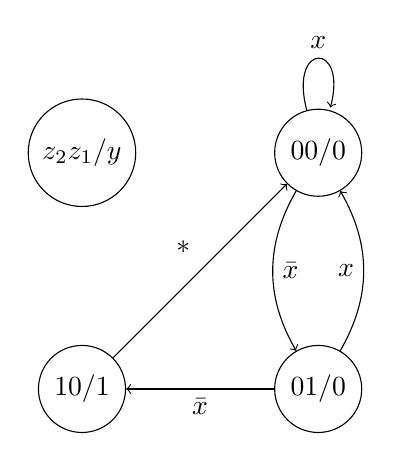
\begin{tikzpicture}[->,auto,node distance=3cm,main node/.style={circle,draw}]
          \node[main node] (-1) {$z_2z_1/y$};
          \node[main node] (0) [right of=-1]{00/0};
          \node[main node] (1) [below of=0] {01/0};
          \node[main node] (2) [left of=1] {10/1};

          \path[every node]
            (0) edge [bend right] node {$\bar x$} (1)
            (0) edge [loop above] node {$x$} (0)
            (1) edge [bend right] node {$x$} (0)
            (1) edge [] node {$\bar x$} (2)
            (2) edge node {*} (0);
        \end{tikzpicture}
      \end{center}
      \begin{enumerate}
        \item Ist das Schaltwerk vom Typ Moore oder Mealy?
        \item Tragen Sie die Ausgabewerte der Schaltfunktionen für die Ausgabe $y$ und den Folgezustand ($z_1^+, z_2^+$) in eine Funktions- \& KV-Tabelle ein.
        \item Übertragen Sie die Tabellenwerte in KV-Diagramme für $z_1^+, z_2^+, y$.
        \item Geben Sie minimale Ausdrücke für die Schaltfunktionen an.
      \end{enumerate}

    \subsection{Codierung}
      \begin{enumerate}
        \item Geben Sie einen Code mit vier Codeworten an, deren (paarweise) Hammingdistanz mindestens 4 ist.
        \item Wieviele Fehler innerhalb eines Codewortes lassen sich mit ihrem Code erkennen?
        \item Wieviele Fehler innerhalb eines Codewortes lassen sich mit ihrem Code korrigieren?
      \end{enumerate}

    \subsection{Mikroprogrammierung}
      Schreiben Sie für eine Stack- \& eine 3-Adress-Maschine mit Load-Store Befehlssatz, jeweils ein Programm zur Berechnung des folgenden Ausdrucks:
      \begin{center}
        $W = A + B - C^2$
      \end{center}
      $W, A, B$ und $C$ sind dabei als Speicheradressen der Operanden zu interpretieren. Die Werte an den Adressen $A, B$ und $C$ sollen vom Programm nicht modifiziert werden. Falls Sie temporäre Variablen benötigen, können Sie die Speicheradressen $D, E, ..., V$ benutzen. Dabei bedeutet $M$ jeweils eine Speicheradresse, $TOS$ steht für "Top of Stack" und $rX, rY, rZ$ bezeichnen je eines von 16 Universalregistern ($r0, ..., r15$) der 3-Adress-Maschine.

        \begin{tabular}{cc}
          Stack-Maschine&3-Address Maschine\\
          \begin{tabular}{|r|l|}
            \hline
            PUSH M&push; TOS=MEM[M]\\
            POP M&MEM[M]=pop; pop\\
            ADD&tmp=TOS; pop; TOS=tmp+TOS\\
            SUB&tmp=TOS; pop; TOS=tmp-TOS\\
            MUL&tmp=TOS; pop; TOS=tmp*TOS\\
            DIV&tmp=TOS; pop; TOS=tmp/TOS\\
            \hline
          \end{tabular}&
          \begin{tabular}{|r|l|}
            \hline
            LOAD rX, M & rX = M\\
            STORE M, rX & M = rX\\
            MOV rX, rY & rX = rY\\
            ADD rX, rY, rZ & rX = rY + rZ\\
            SUB rX, rY, rZ & rX = rY - rZ\\
            MUL rX, rY, rZ & rX = rY * rZ\\
            DIV rX, rY, rZ & rX = rY / rZ\\
            \hline
          \end{tabular}
        \end{tabular}

    \setcounter{subsection}{13}
    \subsection{Betriebssysteme}
      Beantworten Sie schriftliche Fragen zu Betriebssystem-relevanten Themen. Dies können Inhalte, Eigenschaften oder Zusammenhänge sein. Es genügt eine Aufzählung von Schlüsselworten; Textantworten sollen kurz ausfallen: wenige Sätze, <5 Textzeilen!
      \begin{enumerate}
        \item Nennen Sie drei Aufgaben von Betriebssystemen?
        \item Was ist Scheduling?
        \item Was haben Prozesse mit Threads zu tun?
        \item Welche Mechanismen implementieren Virtual Memory?
      \end{enumerate}

  \section{Ersttermin}
    \setcounter{subsection}{3}
    \subsection{IEEE-754}
      Gegeben seien die folgenden zwei Zahlen im IEEE-754 Format mit einfacher Genauigkeit (1-bit für das Vorzeichen, 8-bit für den Exponenten und 7-bit für die Mantisse)
      \begin{center}
        $A = (0|00011010|1000000)$\\
        $B = (0|11100101|0100011)$
      \end{center}
      \begin{enumerate}
        \item Berechnen Sie $C = A \cdot B$ im IEEE-754 Format.
        \item Wie lauten die Zahlen $A, B$ und $C$ im Dezimalsystem? Sehr große und sehr kleine Werte dürfen auch wie folgt dargestellt werden: $<s>*<Wert> \hat{} <Exponenten>$
      \end{enumerate}

    \subsection{Codierung}
      \begin{enumerate}
        \item Geben Sie einen zyklisch einschrittigen Code mit 10 Codewörtern an, von denen eines $1110$ ist.
        \item Kann ein zyklisch einschrittiger Code eine ungerade Anzahl an Codewörtern enthalten? Begründen Sie.
      \end{enumerate}

  \section*{Multiple Choice}\label{sec:mc}\addcontentsline{toc}{section}{\nameref{sec:mc}} % TODO: verify
    \begin{enumerate}
      \item Für Zahlen im Zweierkomplement gilt das:
        \begin{itemize}
          \item Kommutativgesetz \checkmark
          \item Distributivgesetz \checkmark
          \item Assoziativgesetz \checkmark
        \end{itemize}
      \item Für IEEE-754 Gleitkommazahlen gilt das
        \begin{itemize}
          \item Kommutativgesetz \checkmark
          \item Assoziativgesetz
          \item Distributivgesetz
        \end{itemize}
      \item Die UTF-8 Codierung
        \begin{itemize}
          \item wird für Unicode-Zeichen benutzt \checkmark
          \item entspricht in den ersten 128 Zeichen ASCII mit vorangestellter "0" \checkmark
          \item enthält verschiedene Codierungen für Zeilenumbrüche \checkmark
          \item macht die Konvertierung von Zeilenenden beim Datentransfer zwischen Computern überflüssig
          \item ist bei Länge von einem Byte identisch zu iso-8859-1 \checkmark
          \item konvertiert Zeilenumbrüche bei Datentransfer zwischen verschiedenen Betriebsssystemen automatisch
        \end{itemize}
      \item Mit Hilfe der Oder-Verknüpfung können in einem Bitvektor gezielt einzelne Bits
        \begin{itemize}
          \item gelöscht werden
          \item gesetzt werden \checkmark
          \item invertiert werden
        \end{itemize}
      \item Mit einer AND-Verknüpfung können in einem Bitvektor gezielt einzelne Bits
        \begin{itemize}
          \item gelöscht werden \checkmark
          \item gesetzt werden
          \item invertiert werden
        \end{itemize}
      \item Im 2-Komplement ist bei einem Ripple-Carry Addierer ein Carry-Out immer ein Zeichen für
        \begin{itemize}
          \item einen Überlauf \checkmark
          \item einen Unterlauf
          \item den Wechsel zwischen positiven ($\geq 0$) und negativen Zahlenbereichen
        \end{itemize}
      \item Um einen Überlauf bei Zahlen im Zweierkomplement zu erkennen, benötigt man
        \begin{itemize}
          \item nur den Carry-Out
          \item den Carry-Out und die zwei höchsten Bits \checkmark
          \item nur die zwei höchsten Bits
        \end{itemize}
      \item Die Menge der folgenden booleschen Operatoren ist funktional vollständig
        \begin{itemize}
          \item (AND, OR) \checkmark
          \item (AND, NOR) \checkmark
          \item (AND, OR, NOT) \checkmark
          \item (NAND)
        \end{itemize}
      \item Die oberen 8-bit einer Zahl (ganz links stehend) werden bei
        \begin{itemize}
          \item Big Endian Byteordnung an der niedrigsten Adresse gespeichert \checkmark
          \item Big Endian Byteordnung an der höchsten Adresse gespeichert
          \item Little Endian Byteordnung an der höchsten Adresse gespeichert \checkmark
        \end{itemize}
      \item Die unteren 8-bit einer Zahl (ganz rechts stehend) werden bei
        \begin{itemize}
          \item Big Endian Byteordnung an der höchsten Adresse gespeichert \checkmark
          \item Little Endian Byteordnung an der niedrigsten Adresse gespeichert \checkmark
          \item Little Endian Byteordnung an der höchsten Adresse gespeichert
        \end{itemize}
      \item Für RISC-Befehlssätze gilt
        \begin{itemize}
          \item Befehle sind alle gleich lang \checkmark
          \item Typisches Beispiel x86-Befehlssatz
          \item Abarbeitung in mehreren Takten \checkmark
          \item In der Regel: Pipelining \checkmark
        \end{itemize}
      \item Für CISC gilt
        \begin{itemize}
          \item alle Befehle sind gleich lang
          \item Abarbeitung von Befehlen in mehreren Takten \checkmark
          \item Beispiel: MIPS-Befehlssatz
          \item in der Regel: Pipelining
        \end{itemize}
      \item Beim x86-Assembler wird der Stack genutzt für
        \begin{itemize}
          \item die Speicherung von callee-Save Registern \checkmark
          \item die Parameterübergabe \checkmark
          \item Mehrfachverzweigungen
        \end{itemize}
      \item Durch Pipelining
        \begin{itemize}
          \item steigt die Latenz \checkmark
          \item sinkt die Latenz
          \item steigt der Durchsatz \checkmark
          \item sinkt der Durchsatz
          \item wird jede einzelne Assembleroperation schneller abgearbeitet
          \item werden einzelne atomare Operationen schneller abgearbeitet
          \item werden Programme schneller abgearbeitet \checkmark
        \end{itemize}
      \item Für den Cache Speicher gilt
        \begin{itemize}
          \item wird durch die Hardware verwaltet \checkmark
          \item wird von der Software (Betriebssystem, Programmierer, …) verwaltet
          \item beschleunigt den Speicherzugriff
          \item ist für schnell getaktete CPUs unverzichtbar \checkmark
          \item nutzt die räumliche Lokalität von Programmen \checkmark
          \item nutzt die zeitliche Lokalität von Programmen \checkmark
        \end{itemize}
      \item Zu den Aufgaben des Betriebssystems gehört
        \begin{itemize}
          \item das Compilieren von Programmcode
          \item Behandlung von Interrupts bei Benutzereingaben
          \item das Laden von Programmen in den Hauptspeicher \checkmark
          \item das Laden von Programmen aus der Festplatte / SSD
          \item das Verwalten der Prozesse auf dem Computer \checkmark
          \item das Löschen nicht benötigter Dateien auf Festplatten
        \end{itemize}
      \item Bei einem Interrupt
        \begin{itemize}
          \item wechselt das System in den privilegierten Modus \checkmark
          \item verlässt das System den User-Mode
          \item werden geänderte Seiten des Hauptspeichers aktualisiert
          \item findet ein Kontextwechsel statt \checkmark
        \end{itemize}
      \item Semaphore
        \begin{itemize}
          \item sind ein Mechanismus zur Prozesssynchronisation \checkmark
          \item sind ein Mechanismus zur Sicherung der Cache-Kohärenz
          \item sind ein Mechanismus zur Verwaltung beschränkter Ressourcen \checkmark
          \item basieren auf einer booleschen Variablen und zwei atomaren Operationen
          \item basieren auf einer Integer-Variablen und drei atomaren Operationen
        \end{itemize}
      \item Short-Term Scheduling beinhaltet
        \begin{itemize}
          \item die Behandlung von Interrupts \checkmark
          \item die Auswahl des Prozesses, der als nächstes auf der CPU läuft \checkmark
          \item die Auswahl des nächsten Programms
          \item die Auslagerung von Daten in den sekundären Speicher
          \item die Auslagerung von Daten in den Hauptspeicher
          \item die Prozesszustände: Running, Ready und Blocked \checkmark
        \end{itemize}
      \item Virtual-Memory hat zu tun mit
        \begin{itemize}
          \item Segmentierung \checkmark
          \item Swapping \checkmark
          \item Cache-Kohärenz
        \end{itemize}
    \end{enumerate}

  \section*{True/False}\label{sec:tf}\addcontentsline{toc}{section}{\nameref{sec:tf}}
    \begin{enumerate}
      \item Im 1-Komplement wird mit dem Vektor "11...11" die -1 dargestellt.
      \item Der Exponent denormalisierter IEEE-754 Fließkommazahlen ist immer der Vektor "00...00"
      \item Die Entropie H ist unabhängig von der Codierung
      \item Bei einem Code mit Hamming-Abstand von 3 können 2-bit Fehler erkannt werden
      \item Beim Pipelining werden die Maschinenbefehle in einem Takt abgearbeitet
      \item DRAM Speicher ist flächeneffizienter als SRAM
      \item Bei RISC-Architekturen wird der Cache direkt vom Assemblercode angesprochen
      \item Rekursive Funktionsaufrufe setzen einen Stack voraus
      \item Durch den x86-Assembler werden Schleifen immer in bedingte Sprünge übersetzt
      \item Beim Symmetric Multiprocessing muss der Programmierer für die Datenkonsistenz sorgen, wenn mehrere Prozesse über den Speicher kommunizieren.
    \end{enumerate}

\end{document}
